\documentclass[11pt,a4paper]{article}

% Packages
\usepackage[utf8]{inputenc}
\usepackage[spanish, es-tabla, es-lcroman]{babel}
\usepackage{caption}
\usepackage{listings}
\usepackage{adjustbox}
\usepackage[shortlabels]{enumitem}
\usepackage{boldline}
\usepackage{amssymb, amsmath}
\usepackage[margin=1in]{geometry}
\usepackage{xcolor, color}
\usepackage{soul}
\usepackage{epstopdf}
\usepackage{hyperref}
\hypersetup{
     colorlinks   = true,
}

% Meta
\title{\textbf{ESTRUCTURA DE DATOS}\\
	   \textit{Práctica 1. Eficiencia de algoritmos}\\
	   \large \vspace{0.25em} Doble Grado de Informática y Matemáticas}
\author{Antonio Coín Castro\\ José María Martín Luque}
\date{\today}

% Custom
\providecommand{\abs}[1]{\lvert#1\rvert}
\setlength\parindent{0pt}
\definecolor{Light}{gray}{.90}
\definecolor{mygreen}{rgb}{0,0.6,0}
\definecolor{mygray}{rgb}{0.5,0.5,0.5}
\definecolor{mymauve}{rgb}{0.58,0,0.82}
\renewcommand\labelenumi{(\emph{\roman{enumi})}}
\newcommand{\bm}[1]{\boldsymbol{#1}}

\lstset{literate=   % listings config
  {á}{{\'a}}1 {é}{{\'e}}1 {í}{{\'i}}1 {ó}{{\'o}}1 {ú}{{\'u}}1
  {Á}{{\'A}}1 {É}{{\'E}}1 {Í}{{\'I}}1 {Ó}{{\'O}}1 {Ú}{{\'U}}1
  {à}{{\`a}}1 {è}{{\`e}}1 {ì}{{\`i}}1 {ò}{{\`o}}1 {ù}{{\`u}}1
  {À}{{\`A}}1 {È}{{\'E}}1 {Ì}{{\`I}}1 {Ò}{{\`O}}1 {Ù}{{\`U}}1
  {ä}{{\"a}}1 {ë}{{\"e}}1 {ï}{{\"i}}1 {ö}{{\"o}}1 {ü}{{\"u}}1
  {Ä}{{\"A}}1 {Ë}{{\"E}}1 {Ï}{{\"I}}1 {Ö}{{\"O}}1 {Ü}{{\"U}}1
  {â}{{\^a}}1 {ê}{{\^e}}1 {î}{{\^i}}1 {ô}{{\^o}}1 {û}{{\^u}}1
  {Â}{{\^A}}1 {Ê}{{\^E}}1 {Î}{{\^I}}1 {Ô}{{\^O}}1 {Û}{{\^U}}1
  {œ}{{\oe}}1 {Œ}{{\OE}}1 {æ}{{\ae}}1 {Æ}{{\AE}}1 {ß}{{\ss}}1
  {ű}{{\H{u}}}1 {Ű}{{\H{U}}}1 {ő}{{\H{o}}}1 {Ő}{{\H{O}}}1
  {ç}{{\c c}}1 {Ç}{{\c C}}1 {ø}{{\o}}1 {å}{{\r a}}1 {Å}{{\r A}}1
  {€}{{\EUR}}1 {£}{{\pounds}}1 {ñ}{{\~{n}}}1
}

\lstset{    %listings config
  language=C++,
  belowcaptionskip=1\baselineskip,
  breaklines=true,
  frame=L,
  xleftmargin=0.5in,
  %otherkeywords={},
  showstringspaces=false,
  backgroundcolor=\color{white},
  basicstyle=\footnotesize\ttfamily,
  keywordstyle=\bfseries\color{purple!90!black},
  commentstyle=\itshape\color{gray!85!},
  identifierstyle=\color{blue!80!black},
  stringstyle=\color{green!60!black},
}

\newcommand\ddfrac[2]{\frac{\displaystyle #1}{\displaystyle #2}}

% Environments

\begin{document}
\maketitle

\section*{Condiciones de ejecución.}

Dado que en los siguientes ejercicios hablaremos de la eficiencia de distintos programas, conviene detallar las condiciones en las que se han llevado a cabo las pruebas. \\

\textbf{Hardware:} Apple MacBook Pro 13" mid 2015, Intel(R) Core(TM) i5-5257U CPU @ 2.70GHz, 8GB RAM. \\
\textbf{Sistema Operativo:} macOS Sierra 10.12.1 beta (16B2327e). \\
\textbf{Compilador:} clang-800.0.38 \\
\textbf{Opciones de compilación:} -Wall -g

\section*{Ejercicio 1.}
En este ejercicio, comprobaremos tanto la eficiencia teórica como la eficiencia empírica del algoritmo de ordenación \emph{burbuja}:

\begin{lstlisting}[numbers=left]
void ordenar_burbuja(int *v, int n)
{
  for (int i=0; i<n-1; i++)
    for (int j=0; j<n-i-1; j++)
      if (v[j]>v[j+1]) {
        int aux = v[j];
        v[j] = v[j+1];
        v[j+1] = aux;
      }
}
\end{lstlisting}

Comencemos analizando la eficiencia teórica del algoritmo, en el caso peor. Veamos primero el coste en operaciones elementales (OE) de cada línea:\\

\textbf{Línea 3.} Hay 5 OE: una asignación, una resta, una comparación y un incremento(incremento + asignación).

\textbf{Línea 4.} Hay 6 OE: igual que la línea anterior, pero se realizan dos restas.

\textbf{Línea 5.} Hay 4 OE: dos accesos a un vector, una suma y una comparación.

\textbf{Línea 6.} Hay 2 OE: asignación y acceso al vector.

\textbf{Línea 7.} Hay 4 OE: dos accesos, suma y asignación.

\textbf{Línea 8.} Hay 3 OE: acceso, suma y asignación.\\

Entonces, la eficiencia del algoritmo es:

$$ T(n) = 1+ \sum_{i=0}^{n-2} \left( 4 + 1 + \sum_{j=0}^{n-i-2} 18 \right) = 1+ \sum_{i=0}^{n-2} \left( 5 + 18(n-i-1) \right) = 1 + \sum_{i=0}^{n-2} 18n\ - \sum_{i=0}^{n-2} 18i\ - \sum_{i=0}^{n-2} 13 = $$ $$ = 1 + 18n(n-1) - 18 \left( \frac{0 + (n-2)}{2} \cdot (n-1) \right) - 13(n-1) = \frac{18}{2}n^2 - \frac{111}{2} n - \frac{21}{2}.$$

Por tanto, afirmamos que $T(n) \in O(n^2)$, y el algoritmo de ordenación burbuja es de orden de eficiencia $O(n^2)$.\\

Ahora creamos un programa de prueba para analizar la eficiencia empírica, haciendo uso de la biblioteca \emph{ctime} del lenguaje C++:

\lstinputlisting{burbuja.cpp}

Al analizar la eficiencia empírica del algoritmo, obtenemos la siguiente gráfica:\\

\begin{center}
	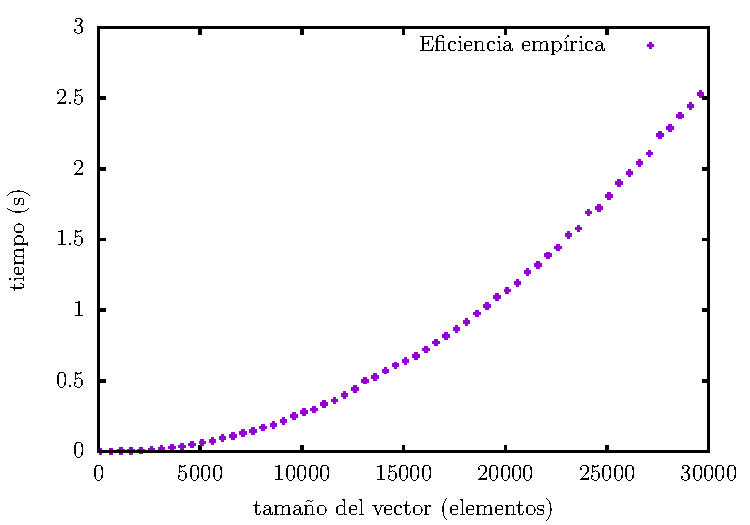
\includegraphics{img/tiempos_burbuja.pdf}
\end{center}

Si representamos superpuestas la función de la eficiencia teórica y la empírica, obtenemos lo siguiente:\\

\begin{center}
	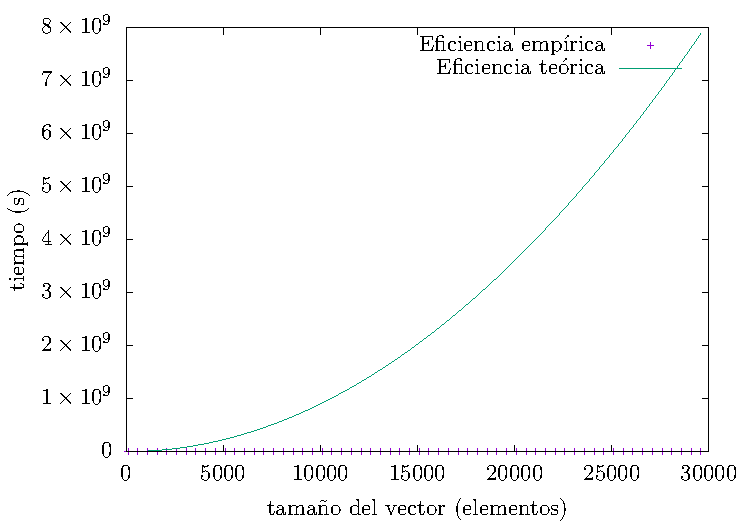
\includegraphics{img/tiempos_burbuja_teorica_superpuesta.pdf}
\end{center}

Observamos que, aunque la curva de la eficiencia teórica tiene la misma forma que la nube de puntos obtenidas experimentalmente, ambas curvas no coinciden al representarlas superpuestas. Esto se debe a que las constantes no coinciden, pues el costo de una operación elemental, e incluso el tiempo total de ejecución del algoritmo, dependen de las condiciones particulares de la máquina en la que se ejecuta.

\section*{Ejercicio 2.}
Veamos que podemos ajustar, mediante \textit{gnuplot}, los puntos obtenidos al analizar la eficiencia empírica en una función de la forma $f(n) = an^2 + bn + c$.\\

En efecto, obtenemos que la función en cuestión es: $$\bm{f(n) = 3.03496^{-9}n^2 - 3.50199^{-6} n + 0.00221794}.$$ Observamos que las constantes obtenidas son mucho más pequeñas que las calculadas para la eficiencia teórica. La representación gráfica es la siguiente, que ya si se ajusta mucho mejor a la nube de puntos:

\begin{center}
	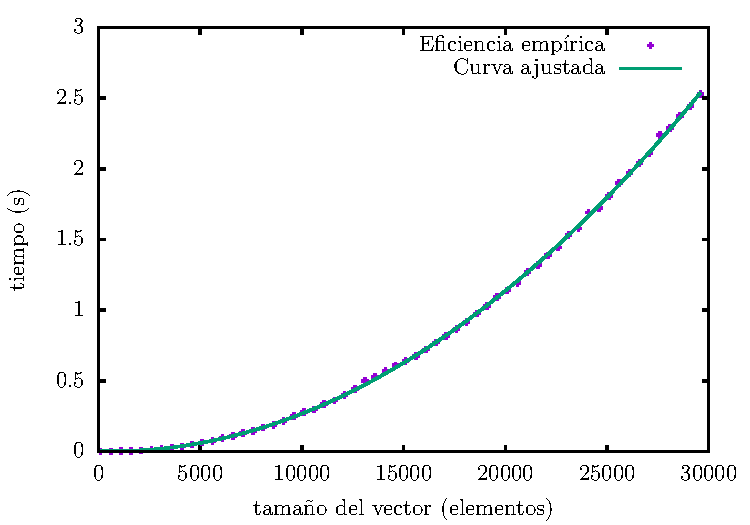
\includegraphics{img/tiempos_burbuja_ajustado.pdf}
\end{center}

\section*{Ejercicio 3.}

\textbf{a)} En este primer apartado, describiremos el funcionamiento del algoritmo proporcionado en el archivo $ejercicio\_desc.cpp$.\\

Se trata de un algoritmo de \textbf{búsqueda binaria}, donde dado un vector $v$ de $n$ elementos enteros, busca el entero $x$ en él. Para ello, se pasan como parámetros el inicio \textit{(inf)} y el final (\textit{sup}) de dicho vector. La función devuelve la posición donde se ha encontrado el elemento, o $-1$ si no estaba en el vector.\\

Para el correcto funcionamiento del algoritmo, es imprescindible que el vector esté \textbf{ordenado}, pues el procedimiento es el siguiente:

\begin{enumerate}
\item Se establece la posición $med = (inf+sup)/2$.
\item Se comprueba si el elemento $x$ está en la posición $med$.
\item Si está, hemos acabado. Si no está, se comprueba si el elemento $v[med]$ es mayor o menor que $x$.
    \begin{itemize}
    \item Si $v[med] < x$, actualizamos $inf = med + 1$.
    \item Si $v[med] > x$, actualizamos $sup = med - 1$.
    \end{itemize}
\item Repetimos el proceso, hasta encontrar el elemento, o concluir que no está en el vector.
\end{enumerate}

En resumen, el procedimiento se basa en dividir el vector original por la mitad, y si no está ahí el elemento buscado, nos quedamos únicamente con el sub-vector donde se puede encontrar dicho elemento (recordemos que el vector está ordenado). Repitiendo el proceso, acabaremos encontrando el elemento, o descubriendo que no está en el vector, cuando ya no se puedan hacer más divisiones.\\

\textbf{b)} Para el cálculo de la eficiencia teórica de la \textit{búsqueda binaria}, nos basamos en el hecho de que se divide sucesivamente en dos un vector de tamaño $n$. En el caso peor, el proceso continuará hasta que no se puedan hacer más divisiones del vector.\\

Por definición, el número máximo de veces que se puede dividir por la mitad un vector de tamaño $n$ es $\log_2 (n)$ veces. Para ilustrarlo, consideramos un vector de $n$ elementos. Sabemos que tras $m$ divisiones, el número de elementos restantes será, como mucho, $\left[\frac{n}{2^m}\right]$, y se detendrá cuando dicho número sea menor que 1. Aplicando logaritmos, se tendría que $\log_2 (n) < m$.\\

Como el resto de operaciones son elementales ($O(1)$), concluímos que la eficiencia del algoritmo es logarítmica, es decir, $T(n) \in O(\log (n))$.\\

\textbf{c)} Para analizar la eficiencia empírica, no podemos simplemente repetir el proceso que hemos seguido anteriormente. Si lo hacemos así, obtendremos una gráfica que es prácticamente horizontal. \\

Esto ocurre porque el algoritmo es tan rápido que es imposible apreciar cambios en el tiempo de ejecución para vectores de tamaño mayor. Por tanto, para analizar empíricamente la eficiencia de este algoritmo debemos ejecutarlo más de una vez por cada tamaño del vector. En nuestro caso lo hemos ejecutado 1000 veces por cada tamaño, obteniendo la siguiente gráfica:

\begin{center}
	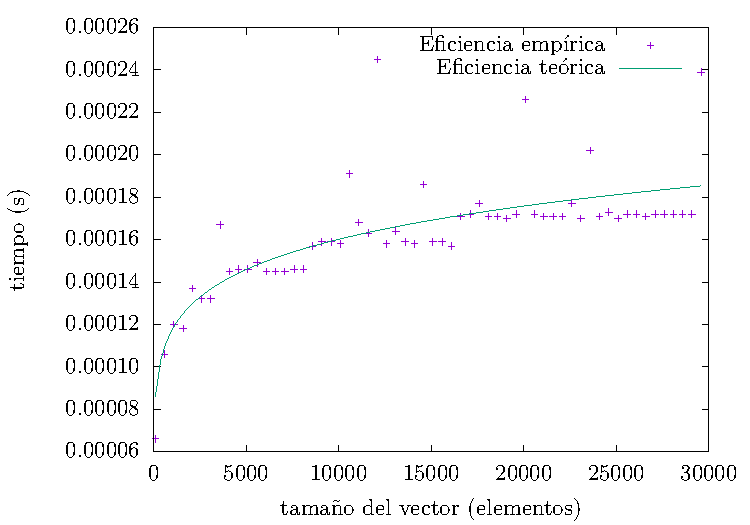
\includegraphics{img/tiempos_binaria.pdf}
\end{center}

Ajustando la nube de puntos a la función exponencial $f(n) = {4.63148 \cdot 10^{-5}n}^{0.134689}$ , se puede observar claramente que la eficiencia empírica describe una gráfica de forma logarítimica, coincidiendo así con nuestros resultados teóricos.

\section*{Ejercicio 4.}

\textbf{a)} Para este apartado, construimos un vector ordenado para representar el caso mejor. Usaremos, por ejemplo, el siguiente código, y elegiremos $vmax > tam$:

\begin{lstlisting}
  // Generación del vector ordenado
  int *v=new int[tam];       // Reserva de memoria
  v[0] = 0;
  for (int i=1; i<tam; i++)  // Recorrer vector
    v[i] = v[i-1] + 1;    // Generar vector ordenado
\end{lstlisting}
\hfill \\
La gráfica que representa la eficiencia empírica es la siguiente:

\begin{center}
	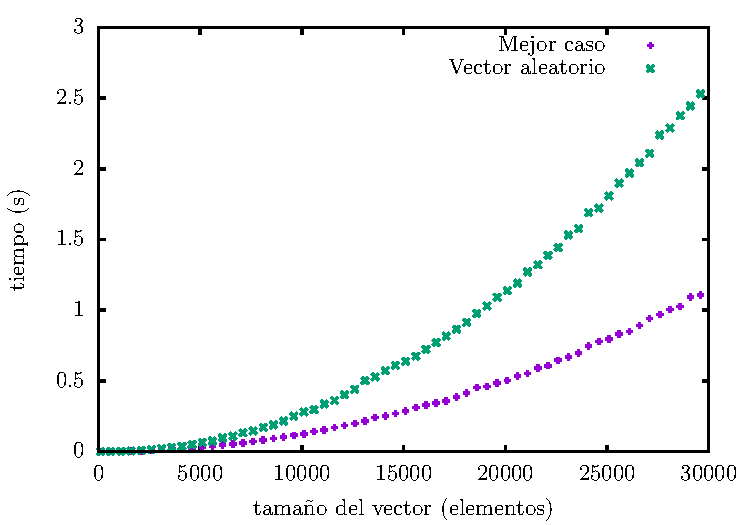
\includegraphics{img/tiempos_burbuja_mejor_caso.pdf}
\end{center}

Como se puede observar, el tiempo de ejecución es mucho menor para el mejor caso que para el vector con los elementos generados aleatoriamente.\\

\textbf{b)} Para este apartado, construimos un vector ordenado en orden inverso, para representar el caso peor. Usaremos, el siguiente código:

\begin{lstlisting}
  // Generación del vector ordenado
  int *v=new int[tam];       // Reserva de memoria
  v[0] = vmax;
  for (int i=1; i<tam; i++)  // Recorrer vector
    v[i] = v[i-1] - 1;    // Generar vector ordenado inversamente
\end{lstlisting}
\hfill \\
La gráfica que representa la eficiencia empírica es la siguiente:

\begin{center}
	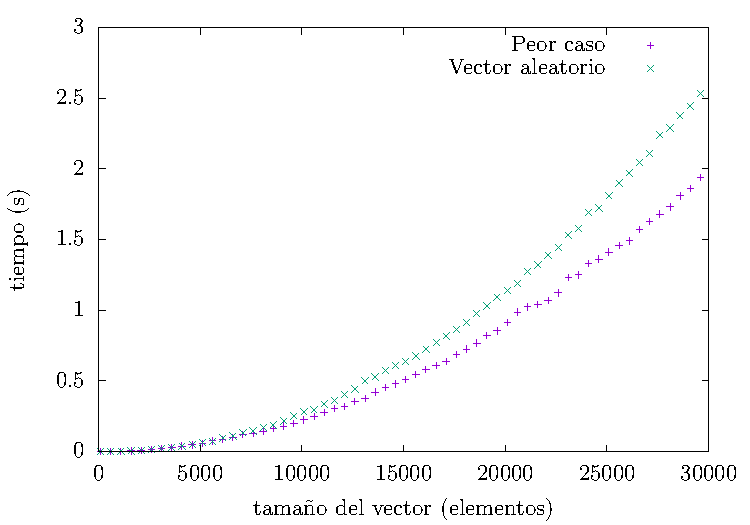
\includegraphics{img/tiempos_burbuja_peor_caso.pdf}
\end{center}

\hypersetup{linkcolor=green}

Observando esta gráfica nos damos cuenta de algo extraño. A pesar de encontrarnos en el 'caso peor', la ordenación de este vector es más rápida que la del vector aleatorio. ¿Por qué? La respuesta a este misterio la encontramos aquí: \href{http://stackoverflow.com/questions/11227809/why-is-it-faster-to-process-a-sorted-array-than-an-unsorted-array}{Why is it faster to process a sorted array than an unsorted array?} Cada vez que hay un salto condicional en una serie de instrucciones los procesadores sufren retardos, debido a que la condición de salto no se evalúa en el acto. Por este motivo, los procesadores cuentan con un circuito llamado \textbf{predictor de saltos} cuyo cometido es analizar el comportamiento de los saltos anteriores para intentar predecir los siguientes. En nuestro caso, dado que el vector con el que trabajamos está ordenado en su totalidad de forma decreciente, el procesador lo tiene fácil para predecir el salto que debe dar. Esto no ocurre en el vector generado aleatoriamente, por lo que el tiempo de ejecución de nuestro 'caso peor' es realmente menor que el del vector aleatorio.

\section*{Ejercicio 5.}

Consideramos la siguiente representación alternativa del algoritmo de ordenación \textbf{burbuja}:

\begin{lstlisting}
void ordenar(int *v, int n) {
    bool cambio=true;
    for (int i=0; i<n-1 && cambio; i++) {
        cambio=false;
        for (int j=0; j<n-i-1; j++)
            if (v[j]>v[j+1]) {
            cambio=true;
            int aux = v[j];
            v[j] = v[j+1];
            v[j+1] = aux;
        }
    }
}
\end{lstlisting}

En esta versión, se ha añadido una variable que permite saber si, en una iteración del bucle externo, no se ha producido un cambio en el vector. Si esto ocurre, el vector ya está ordenado, y no hay que continuar.\\

Si realizamos un estudio teórico de la eficiencia en el mejor caso, es decir, cuando el vector de entrada está ya ordenado, nos damos cuenta rápidamente de que el orden de eficiencia es linear, es decir, $T(n) \in O(n)$. Esto es así porque tan sólo habría que recorrer una vez $n-1$ elementos del vector, hasta darse cuenta de que está ordenado.\\

Analicemos ahora la eficiencia empírica de este algoritmo en el caso mejor. Veamos la gráfica asociada:

\begin{center}
	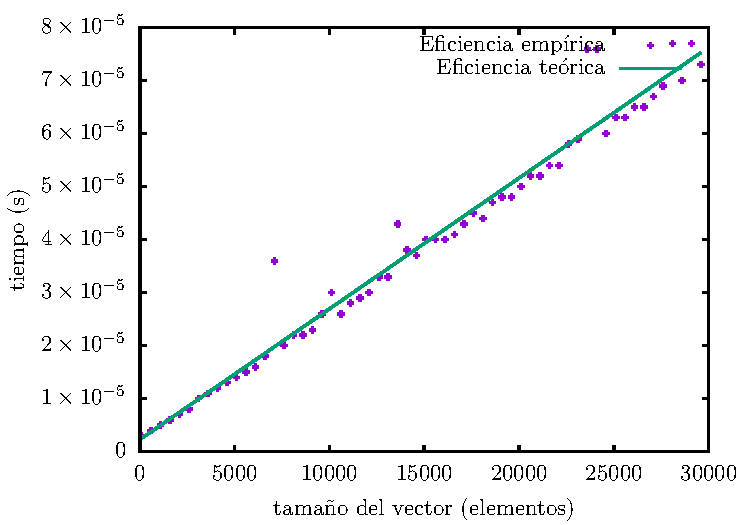
\includegraphics{img/tiempos_burbuja_optimizado.pdf}
\end{center}

Como podemos observar, el orden de eficiencia es efectivamente lineal, con una función de ajuste $f(n) = 2.46724 \cdot 10^{-9}n + 2.26147 \cdot 10^{-6}$, tal y como había predicho nuestro estudio teórico.

\section*{Ejercicio 6.}

Compilando el algoritmo de la burbuja con la opción \textit{-O3} conseguimos que el compilador optimice el código de nuestro programa. Así, midiendo el tiempo de ejecución para distintos tamaños de vector y comparándolo con el que obtuvimos en el ejercicio 1, conseguimos la siguiente gráfica:

\begin{center}
	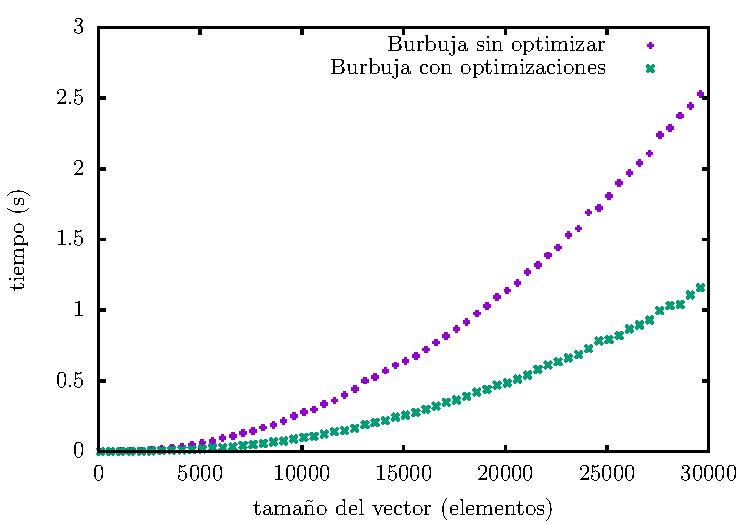
\includegraphics{img/tiempos_burbuja_opt_compilador.pdf}
\end{center}

Podemos observar claramente que el programa con las optimizaciones es mucho más rápido que sin ellas, como era de esperar.

\end{document}
